\section{Introduction:}
Le filtre dit de Kalman a fait l'objet de plusieurs publications fondatrices entre 1958 et 1961, de plusieurs auteurs (notamment Bucy et R.E. Kalman \cite{Kalman1960a, Kalman1961}) mais seul Kalman est finalement passé à la postérité. Il sert à l'estimation dans le temps de la valeur de variables aléatoires gaussiennes, en fonction de valeurs mesurées et d'un modèle d'évolution temporelle. Comme de nombreux filtres bayésiens, il fonctionne en deux étapes, l'état futur du filtre est prédit, puis comparé à la nouvelle mesure, ce qui permet finalement d'en estimer un état corrigé. 

\section{Fonctionnement:}
Une prédiction de l'état futur des variables que l'on cherche à estimer est tout d'abord réalisée, à partir de l'état précédent, d'une fonction de propagation et de paramètres de contrôle éventuels qui influent sur l'évolution prévisible de la variable. Cet état est ensuite rapproché de la nouvelle observation, grâce à une fonction de mesure qui permet d'obtenir à partir de l'état prédit la mesure correspondante (cette fonction est simplement l'identité si l'on est capable de mesurer tous les éléments du vecteur d'état). On peut alors calculer l'innovation, c'est à dire la différence entre la mesure prédite et celle mesurée, et corriger la prédiction pour obtenir une estimation de l'état courant (mis à jour). Ces étapes sont décrites schématiquement sur la figure \ref{fig:ch4_kalman_overview}. Ce filtre est itératif, la prise en compte de l'historique des mesures étant contenue dans ces deux étapes (on suppose que l'état estimé est descriptible par une chaîne de Markov de rang 1).\\

\begin{figure}
	\centering
	\includegraphics[width=\textwidth]{Chapter4/graphics/kalman_filter_overview.png}
	\caption{Schéma de principe d'un filtre de Kalman. Les rectangles représentent des fonctions, les états seuls représentent des vecteurs de variables aléatoires}
	\label{fig:ch4_kalman_overview}
\end{figure}

\section{Restrictions:}
Le filtre de Kalman suppose tout d'abord que les étapes de propagation et de mesure sont linéaires, c'est à dire que la probabilité de transition et la probabilité de mesure doivent être des fonctions affines. Il suppose par ailleurs que les variables aléatoires que l'on cherche à estimer sont distribuées selon une loi normale. Cet algorithme fonctionne en propageant les deux premiers moments statistiques des variables considérées, soit la moyenne et la variance. Une distribution gaussienne est entièrement décrite par ces deux moments, le filtre de Kalman en fournit donc une propagation exacte (dans la limite de systèmes linéaires et purement gaussiens donc, et en supposant que tous les paramètres soient parfaitement connus).

\section{Équations:}
On décrit dans la suite les étapes de propagation du filtre. On note $\mu$ la valeur moyenne estimée, $\Sigma$ la covariance de la variable estimée, $u$ le vecteur des paramètres de contrôle et $z$ le vecteur observation. Les équations suivantes décrivent une itération complète entre les pas de temps $t-1$ et $t$. Les équations \ref{eq:KF_pred1} et \ref{eq:KF_pred2} décrivent donc l'étape de prédiction, le calcul du gain ayant lieu en \ref{eq:KF_KG}, tandis que les étapes de mise à jour sont \ref{eq:KF_up1} et \ref{eq:KF_up2}, et peuvent être rapprochées de la figure \ref{fig:ch4_kalman_overview}: 

\begin{enumerate}
	\item{\emph{Prédiction:}\\}
	On décrit par $\bar{\mu}$ et $\bar{\Sigma}$ l'état prédit, par la matrice $A$ le modèle de propagation de l'état estimé (associé au bruit additif $R$) et par la matrice $B$ la contribution (linéaire) du contrôle à l'état estimé.
	\begin{align}
		\bar{\mu}_t    	&= A_t \mu_{t-1} + B_t u_t \label{eq:KF_pred1}\\ 
		\bar{\Sigma}_t 	&= A_t \Sigma_t A_t^T + R_t \label{eq:KF_pred2}\\
	\end{align}
	
	\item{\emph{Calcul du gain de Kalman:}\\}
	On note $C$ la matrice décrivant la relation (linéaire) entre la mesure et la variable estimée, et $Q$ la matrice de covariance décrivant le bruit additif de mesure. La matrice $K_t$ est souvent appelée "gain de Kalman".
	\begin{align}
		K_t			  	&= 	\bar{\Sigma}_t C_t^T \left( C_t \bar{\Sigma}_t  C_t^T  + Q_t\right)^{-1} \label{eq:KF_KG} \\
	\end{align}	
	
	\item{\emph{Mise à jour:}\\}
	La valeur $z_t - C_t \bar{\mu_t}$ est souvent appelée \emph{innovation}.
	\begin{align}
		\mu_t 			&= \bar{\mu}_t + K_t \left(z_t - C_t \bar{\mu_t} \right) 	\label{eq:KF_up1}\\
		\Sigma_t		&= \left( I - K_t C_t \right) \bar{\Sigma}_t 							\label{eq:KF_up2}\\
	\end{align}
\end{enumerate}

\section{Complexité algorithmique:}
Dans le cas de vecteurs d'état de petite dimensions, le filtre de Kalman est très rapide à mettre en œuvre et ne présente pas de difficultés particulières. Les vecteurs de très grande dimensions, qui peuvent par exemple être présents dans les applications de SLAM peuvent en revanche souligner un point critique. L'essentiel de la complexité calculatoire est dans ce cas contenue dans l'inversion d'une matrice analogue à une covariance dont la taille dépend linéairement du nombre $n$ de variables estimées. Le coût de l'inversion d'une matrice de taille $m$ est de l'ordre de $O(m^{2.4})$ (Thrun, \cite{Thrun2005}), et il s'agit en général du facteur limitant dans la prise en compte de grands systèmes. 